\documentclass[../../InformazioneQuantistica.tex]{subfiles}

\begin{document}
\lesson{5 \greendot}{13/3/2019}

\onlyinsubfile{
\section{Note organizzative}
$2$ visite in laboratorio organizzate in turni (saranno organizzati via Moodle). Possibili settimane: Giovedì 10:30, Venerdì 14:00, tra il 4-5 aprile e il 18-(19) aprile (da definire).\\
Per entrare in laboratorio bisogna seguire un corso online di sicurezza, e firmare una certificazione da consegnare all'entrata dei laboratori. Il link sarà inserito a breve su Moodle.
}

\chapter{Stati e misure}
\section{Matrici densità}
In questa sezione ci occuperemo di introdurre una notazione più avanzata e flessibile per trattare gli \textbf{stati} di un sistema quantistico nella loro più ricca generalità.\\
Non sempre, infatti, è possibile caratterizzare un sistema con una precisa funzione d'onda, dato che ciò comporta possedere la \textit{massima informazione} possibile (stato puro). Spesso si ha a che fare con incertezze o informazioni parziali (stati misti), e saper trattare tali frequenti situazioni permette di accedere ad un insieme di possibilità computazionali molto più ampio.

\subsection{Misture statistiche}
Per \textbf{mistura statistica}\index{Mistura statistica}\marginpar{Mistura statistica} si intende un sistema $S$ che è descritto da una funzione d'onda $\ket{\psi_k}$ che \textit{non conosciamo}, scelta in un insieme di $N$ possibilità $\{\ket{\psi_i}\}_{i=1\dots N}$, ciascuna con probabilità (classica) $p_i$ (con $p_i > 0 \> \forall i$ e $\sum_{i=1}^N p_i = 1$).\\

\textbf{Nota}: Una situazione di questo tipo è fondamentalmente differente da quella in cui il sistema si trova in una \textit{sovrapposizione} delle $N$ funzioni d'onda (ossia in un $\ket{\Psi} = \sum_{i=1}^N \alpha_i \ket{\psi_i}$), poiché nel caso di mistura statistica le singole $\ket{\psi_i}$ \textbf{non interferiscono} tra loro, cosa che invece succede nel caso di una sovrapposizione.\\

Come possiamo descrivere efficacemente una mistura statistica, in modo da calcolarne valor medi ed evoluzione temporale?\\
Partiamo dalla definizione di \textbf{osservabile} $\hat{A}$ in termini di proiettori $\hat{P}_i$, e cerchiamo di riadattarla alla nuova situazione:
\begin{align}
\hat{A} = \sum_i a_i \hat{P}_i \qquad \hat{P}_i = \ket{a_i}\bra{a_i}
\label{eqn:osservabile-def}
\end{align}
Se $S$ fosse nello stato $\ket{\psi_k}$ potremmo usare direttamente la formula per il valor medio di $\hat{A}$, pari alla combinazione lineare dei valor medi $q_k(i)$ dei singoli proiettori:
\begin{align}
\langle \hat{A} \rangle_{\psi_k} = \sum_i a_i \langle \hat{P}_i \rangle_{\psi_k} = \sum_i a_i\, q_k(i); \qquad q_k(i) = \bra{\psi_k}\hat{P}_i\ket{\psi_k}
\label{eqn:val-medio-psik}
\end{align}
Non sapendo però in quale $\ket{\psi_k}$ si trovi il sistema, dovremo considerare tutte le $N$ possibilità $\{\ket{\psi_k}\}$, pesandole con le rispettive probabilità di occorrenza $p_k$. La media pesata dei valori di aspettazione dell'$i$-esimo proiettore $\hat{P}_i$ nell'\textit{ensemble} dei possibili stati $\{\ket{\psi_k}\}$ viene denotata con $\tilde{P}(i)$. 
\begin{align*}
\tilde{P}(i) = \sum_{k=0}^N p_k \,q_k(i) = \sum_{k=0}^N p_k \bra{\psi_k}\hat{P}_i \ket{\psi_k}
\end{align*}
Sommando allora su tutti i proiettori giungiamo alla formula per il valor medio di $\hat{A}$ della mistura statistica $\{(\ket{\psi_k},p_k)\}$:
\begin{align}
\langle \hat{A} \rangle = \sum_i a_i \tilde{P}(i) = \sum_{k=0}^N p_k \sum_i a_i \bra{\psi_k}\hat{P}_i\ket{\psi_k} = \sum_{k=0}^N p_k \bra{\psi_k}\hat{A}\ket{\psi_k} = \op{Tr}(\bm{\rho} \hat{A})
\label{eqn:traccia-valor-medio}
\end{align}
Dove $\rho$ è detta \textbf{matrice di densità} ed è definita da:\marginpar{Matrice densità}\index{Matrice densità}
\begin{align}
\rho \equiv \sum_{k=1}^N p_k \ket{\psi_k}\bra{\psi_k}
\label{eqn:matrice-density}
\end{align}
Ricordiamo che l'operazione di \textbf{traccia}\index{Traccia} consiste nella somma sugli elementi sulla diagonale della rappresentazione matriciale di $\rho A$ in una qualsiasi base ON $\{\ket{\chi_j}\}$ di $\hs$ (il risultato è indipendente dalla scelta della base):
\begin{align*}
\op{Tr}(B)=\sum_{j=1}^{\op{dim}\hs} \bra{\chi_j}B\ket{\chi_j}
\end{align*}
\begin{expl}
\textbf{Verifichiamo} la formula (\ref{eqn:traccia-valor-medio}). Nel caso $N=0$ avremo una sola possibilità per lo stato $\ket{\psi_0}$, da cui $\rho = p_0\ket{\psi_0}\bra{\psi_0}$ (dove $p_0=1$). Considerando allora una base con $\ket{\chi_1} = \ket{\psi_0}$ si trova:
\begin{align*}
\op{Tr}(\rho A) =
\op{Tr}(p_0\ket{\psi_0}\bra{\psi_0}\hat{A})=\sum_{i=1}^{\op{dim}\hs}p_0 \braket{\chi_i|\psi_0}\bra{\psi_0}\hat{A}\ket{\chi_i}=p_0 \bra{\psi_0}\hat{A}\ket{\psi_0}
\end{align*} 
E il risultato è uguale per ogni altra base ON per le proprietà della traccia. Considerando al posto di $\ket{\psi_0}$ un $\ket{\psi_k}$ generico vale quindi:
\begin{align*}
\op{Tr}(p_k\ket{\psi_k}\bra{\psi_k}\hat{A})=p_k\bra{\psi_k}\hat{A}\ket{\psi_k}
\end{align*}
Perciò possiamo sommare su $k$ per riottenere la (\ref{eqn:traccia-valor-medio}):
\begin{align*}
\sum_{k=0}^N p_k \bra{\psi_k}\hat{A}\ket{\psi_k}=\sum_{k=0}^N\op{Tr(p_k\ket{\psi_k}\bra{\psi_k}\hat{A}}) \underset{(a)}{=} \op{Tr}\left(\sum_{k=0}^{N} p_k \ket{\psi_k}\bra{\psi_k}\hat{A}\right)=\op{Tr}(\rho \hat{A})
\end{align*}
dove in (a) abbiamo infine utilizzato la \textbf{linearità} della traccia.
\end{expl}

\subsection{Evoluzione temporale}
Le singole $\ket{\psi_k}$ evolvono in maniera unitaria:
\begin{align*}
\ket{\psi_k(t)} = U(t-t_0) \ket{\psi(t_0)}
\end{align*}
Sostituendo nella definizione (\ref{eqn:matrice-density}) otteniamo perciò l'\textbf{evoluzione} della matrice densità:
\begin{align*}
\rho(t) = \sum_{k=0}^N p_k \ket{\psi_k(t)}\bra{\psi_k(t)} = \sum_{k=0}^N p_k [U\ket{\psi(t_0)}][\bra{\psi(t_0)}U^\dag] = U \rho_0 U^\dag
\end{align*}

Per gli stati puri $\ket{\psi}$ (che siano nel dominio dell'Hamiltoniana $\hat{H}$ del sistema) vale l'equazione di Schr\"odinger dipendente dal tempo:
\begin{align}
i\hbar \frac{\partial \psi(t)}{\partial t} = \hat{H}\psi(t)
\label{eqn:schrody-temp}
\end{align}

Un'equazione analoga vale per le misture statistiche (dette anche \textbf{stati misti}), e prende il nome di equazione di \textbf{Liouville-von Neumann}.\index{Equazione!Liouville-von Neumann}\marginpar{Equazione di Liouville-von Neumann} La si ricava calcolando la derivata temporale della matrice densità:
\begin{align*}
\dot{\rho}(t) &=\frac{d}{dt} \sum_{k=0}^N p_k \ket{\psi_k}\bra{\psi_k} = \sum_{k=0}^N p_k \left[\left(\frac{d}{dt}\ket{\psi_k}\right) \bra{\psi_k} + \ket{\psi_k}\left(\frac{d}{dt}\bra{\psi_k}\right)\right]=\\
&\underset{(\ref{eqn:schrody-temp})}{=} \frac{1}{i\hbar}(H\rho - \rho H) = \frac{1}{i\hbar}[H,\rho]
\end{align*}
Riarrangiando giungiamo a:
\begin{align*}
i\hbar \frac{d}{dt}\rho(t) =[H,\rho(t)]
\end{align*}
\begin{expl}
Nel dettaglio, questa equazione è valida nella \textbf{visuale di Schr\"odinger}, dove lo stato (rappresentato dalla matrice densità $\rho$) evolve nel tempo, mentre gli operatori che agiscono su di esso no.\\
La natura matriciale di $\rho(t)$, tuttavia, mostra una forte analogia con l'equazione di evoluzione temporale degli operatori $A^{(H)}(t)$ nella \textbf{visuale di Heisenberg} (dove, invece, $\rho$ è indipendente dal tempo):
\begin{align*}
i\hbar\frac{d A^{(H)}}{dt} = -[H,A^{(H)}(t)]
\end{align*}
a meno di una differenza di segno, data dalla diversa visuale.
\end{expl}

\subsection{Proprietà della matrice densità}
La matrice densità $\rho$ gode delle seguenti proprietà:
\begin{enumerate}
\item $\rho$ è \textbf{hermitiana}.\marginpar{Hermitiana}\\
\textbf{Dim}. Sia $\{\ket{i}\}$ una base ON. Scriviamo le $\ket{\psi_k}$ in questa base:
\begin{align}
\ket{\psi_k} = \sum_{i=1}^{\op{dim}\hs} c_i^k \ket{i} \qquad c_i^k \in \bb{C}
\label{eqn:expandi-base}
\end{align} 
Gli elementi di matrice di $\rho$ sono quindi dati da:
\begin{align}\nonumber
\rho_{ij} &= \bra{i}\rho\ket{j} = \sum_{k=0}^N
p_k \braket{i|\psi_k}\braket{\psi_k|j} \underset{(a)}{=} \sum_{k=0}^N p_k \sum_{l,m} c^k_l (c_m^k)^* \underbrace{\braket{i|l}}_{\delta_{il}}\underbrace{\braket{m|j}}_{\delta_{mj}} =\\
&=\sum_{k=0}^N p_k\, c_i^k (c_j^k)^*
\label{eqn:rho-matrix} 
\end{align}
dove in (a) abbiamo usato l'espansione delle $\ket{\psi_k}$ nella base (\ref{eqn:expandi-base}). In altre parole, gli elementi di matrice $\rho_{ij}$ sono prodotti dei coefficienti $i$ e $j$ della rappresentazione di $\ket{\psi_k}$ nella base $\ket{i}$ in cui $\rho$ è scritta, mediati sull'intero ensemble delle $\{\ket{\psi_k}\}$ possibili, con i pesi dati dalle loro probabilità $p_k$. \\
Invertendo $i$ e $j$ e coniugando otteniamo lo stesso risultato:
\begin{align*}
\rho_{ji}^* = \sum p_k (c_j^k)^* c_i^k = \rho_{ij}
\end{align*}
Ne deriva allora che $\rho$ è hermitiana (essendo simmetrica e a dimensione finita\footnote{L'hermitianicità si dimostra anche nel caso di dimensione infinita.}).
\item $\op{Tr}\rho \bm{= 1}$.\marginpar{Traccia unitaria}\\
\textbf{Dim}. Basta fare il conto diretto usando l'espressione (\ref{eqn:rho-matrix}) per gli elementi di matrice:
\begin{align*}
\op{Tr}\rho = \sum_{i=0}^{\op{dim}\hs} \rho_{ii} = \sum_{k=0}^N p_k \left(\sum_{i=0}^{\op{dim} \hs} |c_i^k|^2 \right) \underset{(a)}{=} \sum_{k=0}^N p_k \underset{(b)}{=} 1
\end{align*}
La somma dei $|c_i^k|^2$ su $i$ in (a) è pari a $\norm{\ket{\psi_k}}^2$ (lo si vede usando (\ref{eqn:expandi-base})), che è pari a $1$ per la normalizzazione. In (b) usiamo poi la \textit{convessità} delle $p_k$, che quindi \q{esauriscono tutte le possibilità}, dato che sappiamo con certezza il sistema si trova in uno stato in $\{\ket{\psi_k}\}$ (per come abbiamo definito la mistura statistica).
\item $\rho$ è un operatore \textbf{non-negativo}\marginpar{Non negativa}, cioè $\forall \ket{\psi}$ vale $\bra{\psi}\rho\ket{\psi}\geq 0$.\\
\textbf{Dim}. Per calcolo diretto con una generica $\ket{\varphi}$, usando di nuovo la (\ref{eqn:rho-matrix}):
\begin{align*}
\bra{\varphi}\rho \ket{\varphi} =\ \bra{\varphi}\left(\sum_{k=0}^N p_k \ket{\psi_k}\bra{\psi_k}\right) \ket{\varphi} = \sum_{k=0}^N p_k |\braket{\varphi|\psi_k}|^2 \geq 0
\end{align*}
\end{enumerate}

\subsection{Stati puri e misti}
La matrice di densità $\rho$ può essere usata sia per rappresentare \textbf{stati puri} che \textbf{misture statistiche} (\textbf{stati misti}).\\
\textbf{Riepilogando}, uno stato \textbf{puro} è dato da $\rho$ prodotta da un unico termine:
\begin{align*}
\rho_p &=\ket{\psi}\bra{\psi}
\intertext{Mentre per uno stato \textbf{misto} si ha:}
\rho_m &= \sum_{k=0}^N p_k \ket{\psi_k}\bra{\psi_k}
\end{align*}

Si possono differenziare i due casi notando che il primo è un \textbf{proiettore}, e quindi\marginpar{Differenza tra stati misti e puri} $\rho_p^2 = \rho_p$. Da ciò segue che:
\begin{align*}
\op{Tr} \rho_m^2 < 1 \qquad \op{Tr} \rho_p = 1
\end{align*}
\textbf{Dim.} Eseguiamo il calcolo diretto, usando la base $\{\ket{j}\}$ in cui $\rho$ è diagonale:
\begin{align*}
\rho = \sum_{j=0}^{N} \lambda_j \ket{j}\bra{j} \Rightarrow \rho^2 = \sum_{j,k=0}^N \lambda_j \lambda_k \, \ket{k}\underbrace{\braket{k|j}}_{\delta_{kj}}\bra{j}= \sum_{j=0}^{N} \lambda_j^2 \ket{j}\bra{j}
\end{align*}
Notiamo che:
\begin{align*}
\sum_{j=0}^N \lambda_j = 1; \> \lambda_j \geq 0 \Rightarrow 0\leq \lambda_j \leq 1
\end{align*}
E perciò, in generale:
\begin{align*}
\op{Tr} \rho^2 = \sum_{j=0}^N \lambda_j^2  \leq \sum_{j=0}^N \lambda_j = 1
\end{align*}
E si ha l'uguaglianza solo nel caso specifico in cui $\lambda_{j^*}=1$ per un certo $0 \leq j^* \leq N$, e tutti gli altri $\lambda_{j \neq j^*}=0$, che corrisponde a quello in cui $\rho$ rappresenta uno \textbf{stato puro}. In tutti gli altri casi (\textbf{stati misti}), $\op{Tr}(\rho^2)$ sarà quindi \textit{strettamente} minore di $1$.\\
Per questò la grandezza (misurabile sperimentalmente, dato che $\rho$ è hermitiana, e quindi è un'osservabile) $\op{\textbf{Tr}}\bm{(\rho^2)}$ è detta \textbf{purità}\marginpar{Purità di uno stato $\rho$}\index{Purità} dello stato $\rho$: è massima (pari a $1$) per stati puri, e $0\leq \op{Tr}(\rho^2) < 1$ per stati misti.\\

\textbf{Nota}: l'evoluzione \textbf{unitaria} \textbf{conserva} la purità. Segue che uno stato puro può evolvere unitariamente esclusivamente a stati puri, e allo stesso modo uno stato misto resterà sempre misto (almeno finché il sistema rimane isolato).\\

Nella base $\{\ket{j}\}$ che abbiamo appena considerato, la matrice $\rho$ è diagonale, ma generalmente potremmo scriverla in una qualsiasi altra base ON.\\
Distinguiamo perciò tra gli elementi $\lambda_1 \dots \lambda_N$ sulla diagonale di $\rho$, detti \textbf{termini di popolazione}, e quelli fuori dalla diagonale, detti \textbf{termini di coerenza}.\marginpar{Termini di popolazione/coerenza}\index{Termini di popolazione}\index{Termini di coerenza} Come vedremo nelle prossime sezioni, questi ultimi sono indice delle \textit{correlazioni} tra i singoli stati.\\

\textbf{Nota}: la \q{misurabilità} delle correlazioni dipende quindi dalla base utilizzata. Se la base computazionale è quella che diagonalizza $\rho$, avremo solo termini di popolazione, e nessuna correlazione:
\begin{align*}
\rho = \begin{pmatrix}
\lambda_1 & 0 & \cdots & 0\\
0 & \ddots & 0 & \vdots \\
\vdots & 0  & \ddots &\vdots \\
0 & 0 & 0 & \lambda_N
\end{pmatrix}
\end{align*} 
Tuttavia, come già visto negli esempi di algoritmi, le correlazioni sono molto importanti per la computazione quantistica.

\subsection{Il sistema da 1 qubit}\index{Esempio!Matrice densità di un qubit}
Consideriamo un generico qubit nello \textbf{stato puro} $\ket{\psi}$, che, nella base computazionale $\{\ket{0}, \ket{1}\}$, è dato da:
\begin{align*}
\ket{\psi}=\cos\frac{\theta}{2}\ket{0} + e^{i\varphi}\sin\frac{\theta}{2}\ket{1} = \begin{pmatrix}
\cos\frac{\theta}{2}\\
\sin\frac{\theta}{2}e^{i\varphi}
\end{pmatrix}
\end{align*}
La matrice densità ad esso associata è data da:
\begin{align}
\rho(\theta,\varphi) = \ket{\psi}\bra{\psi}\underset{(a)}{=} \begin{pmatrix}
\cos\frac{\theta}{2}\\
\sin\frac{\theta}{2}e^{i\varphi}
\end{pmatrix}
\begin{pmatrix}
\cos\frac{\theta}{2} & \sin\frac{\theta}{2}e^{\bm{-}i\varphi}
\end{pmatrix} = \begin{pmatrix}
\cos^2 \frac{\theta}{2} & \sin\frac{\theta}{2}\cos\frac{\theta}{2} e^{-i\varphi}\\
\sin\frac{\theta}{2}\cos\frac{\theta}{2} e^{i\varphi} & \sin^2 \frac{\theta}{2}
\end{pmatrix}
\label{eqn:rho-qubit}
\end{align}
\textbf{Nota}: il prodotto tra un ket e un bra in (a) si realizza in notazione matriciale come il prodotto tra un vettore colonna (il ket) e un vettore riga con componenti coniugate (il bra). Questo si ha poiché bra e ket sono collegati da una coniugazione, che corrisponde alla \textit{trasposta coniugata} nel linguaggio delle matrici.\\

Le coordinate $(\theta,\varphi)$ sono le coordinate polari nella sfera di Bloch, e individuano un vettore (\textbf{unitario}) di coordinate cartesiane:
\begin{align}
\begin{pmatrix} x\\y \\z\end{pmatrix} =
\begin{pmatrix} \sin\theta \cos\varphi\\
\sin\theta \sin\varphi\\
\cos\theta
\end{pmatrix}
\qquad x^2+y^2+z^2=1
\label{eqn:versore-coord}
\end{align}
Possiamo allora riscrivere la (\ref{eqn:rho-qubit}) in questa forma, usando formule di bisezione e duplicazione per $\sin$/$\cos$:
\begin{align}\nonumber
 \rho &=
\begin{pmatrix}
\cos^2\frac{\theta}{2} & \frac{1}{2}\sin\theta\,e^{-i\varphi}\\
\frac{1}{2}\sin\theta\, e^{i\varphi} & \sin^2\frac{\theta}{2}
\end{pmatrix} =
\frac{1}{2}
\begin{pmatrix}
1+\cos\theta & \sin\theta(\cos\varphi-i\sin\varphi)\\
\sin\theta(\cos\varphi + i\sin\varphi) & 1-\cos\theta
\end{pmatrix} =\\
&= \frac{1}{2} \begin{pmatrix}
1+z & x-iy\\
x+iy & 1-z
\end{pmatrix} = \frac{1}{2} (\bb{I} + x \hat{\sigma}_x + y \hat{\sigma}_y + z\hat{\sigma}_z)
\label{eqn:rho-matrix-cartesiana}
\end{align}
Nell'ultimo passaggio si è ottenuta un'espansione nella base delle matrici hermitiane $2\times 2$, data da identità e matrici di Pauli $\{\bb{I}, \hat{\sigma}_x, \hat{\sigma}_y, \hat{\sigma}_z\}$, che è molto comoda per i conti (dato che esiste una formula per l'esponenziale di un vettore di Pauli).\\

Ponendo $\vec{r}=(x,y,z)$, il determinante di $\rho$ è dato da: 
\begin{align}
\op{det}\rho = \frac{1}{4}[(1+z)(1-z)-(x+iy)(x-iy)]= \frac{1}{4}(1-\norm{\vec{r}}^2)
\label{eqn:det-rho}
\end{align}

Abbiamo visto che una matrice densità $\rho$ che descrive uno stato puro può essere rappresentata come un vettore $\vec{r}$ che \q{punta} sulla superficie della sfera di Bloch.\\

 \textbf{Estendiamo} ora tale notazione, partendo da un vettore $\vec{r}$ generico.\\
Poiché $\rho$ è hermitiana e non-negativa, ha autovalori reali positivi (al più nulli) e quindi il suo determinante (prodotto degli autovalori) è non negativo:
\begin{align*}
\op{det}\rho \geq 0
\end{align*}
Tale condizione, unita alla (\ref{eqn:det-rho}), porta a $\norm{\vec{r}}\leq 1$.\\

Mostriamo ora che l'uguaglianza $\norm{\vec{r}}=1$ avviene solo quando $\vec{r}$ rappresenta\marginpar{Gli stati puri $\leftrightarrow$ superficie della sfera di Bloch ($\norm{\vec{r}}=1$)} uno \textbf{stato puro}. Sappiamo già che le $\rho$ di stati puri generano vettori $\vec{r}$ unitari (deriva dalla condizione (\ref{eqn:versore-coord})), e manca solo da mostrare il viceversa. Se $\norm{\vec{r}}=1$, si ha per la (\ref{eqn:det-rho}) che $\op{det}\rho = 0$, ma vale sempre $\op{Tr}(\rho)=1$. Detti $\lambda_1$ e $\lambda_2$ gli autovalori di $\rho$, si ha quindi:
\begin{align*}
\begin{cases}
\op{det}\rho = \lambda_1\lambda_2 = 0\\
\op{Tr} \rho = \lambda_1 + \lambda_2 = 1
\end{cases}
\end{align*}
Perciò uno dei due (es. $\lambda_1$) è identicamente $1$, e l'altro è nullo. Ma allora, se $\ket{u}$ è l'autovettore di autovalore $1$, si ha $\rho = \ket{u}\bra{u}$, che rappresenta uno stato puro.\\

Perciò, si ha che tutte le scelte di $\norm{\vec{r}}<1$, che corrispondono ad altrettante possibilità per $\rho$, codificano\marginpar{Stati misti $\leftrightarrow$ $\norm{\vec{r}}<1$} \textbf{stati misti}.\\
Perciò, tra tutte le $\rho$ possibili per un sistema a \textbf{1 qubit} (date da generici vettori nella sfera di Bloch) la maggior parte è prodotta da stati misti (l'interno). Considerare misture statistiche (nella notazione della matrici di densità) permette di sfruttare tale numero molto più ampio di possibilità.\\

\begin{figure}
    \centering
    \tikzset{every picture/.style={line width=0.75pt}} %set default line width to 0.75pt        
\begin{center}
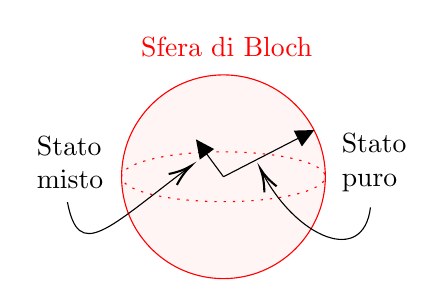
\begin{tikzpicture}[x=0.75pt,y=0.75pt,yscale=-1,xscale=1]
%uncomment if require: \path (0,368); %set diagram left start at 0, and has height of 368

%Shape: Circle [id:dp18999746887747793] 
\draw  [color={rgb, 255:red, 255; green, 0; blue, 0 }  ,draw opacity=1 ][fill={rgb, 255:red, 255; green, 0; blue, 0 }  ,fill opacity=0.04 ] (269.33,171.75) .. controls (269.33,144.64) and (291.31,122.67) .. (318.42,122.67) .. controls (345.52,122.67) and (367.5,144.64) .. (367.5,171.75) .. controls (367.5,198.86) and (345.52,220.83) .. (318.42,220.83) .. controls (291.31,220.83) and (269.33,198.86) .. (269.33,171.75) -- cycle ;
%Straight Lines [id:da7326942600928257] 
\draw    (318.42,171.75) -- (360.39,150.16) ;
\draw [shift={(362.17,149.25)}, rotate = 512.78] [fill={rgb, 255:red, 0; green, 0; blue, 0 }  ][line width=0.75]  [draw opacity=0] (8.93,-4.29) -- (0,0) -- (8.93,4.29) -- cycle    ;

%Curve Lines [id:da9169015177599222] 
\draw    (243.25,184) .. controls (248.7,212.71) and (262.47,196.83) .. (301.56,167.4) ;
\draw [shift={(302.75,166.5)}, rotate = 503.13] [color={rgb, 255:red, 0; green, 0; blue, 0 }  ][line width=0.75]    (10.93,-3.29) .. controls (6.95,-1.4) and (3.31,-0.3) .. (0,0) .. controls (3.31,0.3) and (6.95,1.4) .. (10.93,3.29)   ;

%Curve Lines [id:da8720399522020343] 
\draw    (389.25,186.5) .. controls (385.8,215.07) and (353.25,200.94) .. (336.98,169.45) ;
\draw [shift={(336.25,168)}, rotate = 423.78999999999996] [color={rgb, 255:red, 0; green, 0; blue, 0 }  ][line width=0.75]    (10.93,-3.29) .. controls (6.95,-1.4) and (3.31,-0.3) .. (0,0) .. controls (3.31,0.3) and (6.95,1.4) .. (10.93,3.29)   ;

%Flowchart: Connector [id:dp4640001727103482] 
\draw  [color={rgb, 255:red, 255; green, 0; blue, 0 }  ,draw opacity=1 ][dash pattern={on 0.84pt off 2.51pt}] (269.33,171.75) .. controls (269.33,165.12) and (291.31,159.75) .. (318.42,159.75) .. controls (345.52,159.75) and (367.5,165.12) .. (367.5,171.75) .. controls (367.5,178.38) and (345.52,183.75) .. (318.42,183.75) .. controls (291.31,183.75) and (269.33,178.38) .. (269.33,171.75) -- cycle ;
%Straight Lines [id:da1698778133695058] 
\draw    (318.42,171.75) -- (306.35,155.36) ;
\draw [shift={(305.17,153.75)}, rotate = 413.64] [fill={rgb, 255:red, 0; green, 0; blue, 0 }  ][line width=0.75]  [draw opacity=0] (8.93,-4.29) -- (0,0) -- (8.93,4.29) -- cycle    ;


% Text Node
\draw (320,109) node [color={rgb, 255:red, 255; green, 0; blue, 0 }  ,opacity=1 ] [align=left] {Sfera di Bloch};
% Text Node
\draw (391,165) node  [align=left] {Stato\\puro};
% Text Node
\draw (244.5,165) node  [align=left] {Stato\\misto};


\end{tikzpicture}
\end{center}
    \caption{La sfera di Bloch comprende tutti gli stati possibili per un sistema a $1$ qubit. Gli stati \textit{interni} sono \textbf{stati misti}, mentre quelli \textit{sulla superficie} sono \textbf{stati puri}}
    \label{fig:sfera-bloch-stati}
\end{figure}

In questa notazione vettoriale possiamo visualizzare la genesi di uno stato misto come \textit{somma} di vettori di stati puri opportunamente pesati da probabilità. Il caso più semplice è quello in cui $\vec{r}$ è distribuito uniformemente su tutta la superficie della sfera unitaria, e corrisponde alla \textbf{mistura} di tutti gli stati puri possibili, ossia allo \textbf{stato massimamente misto}. Possiamo calcolare analiticamente la $\rho$ risultante integrando sulla superficie della sfera di Bloch (dove l'integrazione si intende su ciascun elemento di (\ref{eqn:rho-qubit})):
\begin{align*}
\rho = \frac{1}{4\pi}\int_0^{2\pi} d\varphi \int_0^\pi (d\theta \sin\theta) \rho(\theta,\varphi) = \frac{1}{2}\bb{I} = \begin{pmatrix}
\frac{1}{2} & 0 \\ 0 & \frac{1}{2}\end{pmatrix} = \frac{1}{2}\ket{0}\bra{0} + \frac{1}{2}\ket{1}\bra{1}
\end{align*}

\subsection{Sistemi composti}
Nell'ultima sezione abbiamo esaminato un sistema formato da un singolo qubit, notando l'utilità della nuova notazione introdotta.\\
Il principale utilizzo delle matrici densità, tuttavia, si realizza nel considerare \textit{sistemi composti}, tali da codificare $2$ o più qubit.\\
Procedendo con ordine, partiamo dal caso più semplice di \textbf{2 qubit}.\\
Sappiamo che se gli stati del sistema $1$ stanno in uno spazio di Hilbert $\hs_1$ e gli stati del sistema $2$ in $\hs_2$, gli stati del sistema composto si trovano nel prodotto tensore dei due spazi, cioè in:
\begin{align*}
\hs_{12} = \hs_1 \otimes \hs_2
\end{align*}
Una generica funzione d'onda in $\hs_{12}$ si scrive come:
\begin{align*}
\ket{\psi} = \sum_{i,\alpha} c_{i\alpha} \ket{i}_1\ket{\alpha}_2 \qquad \sum_{i,\alpha} |c_{i,\alpha}|^2 = 1
\end{align*}
dove $\{\ket{i}_1\}$ e $\{\ket{\alpha}_2\}$ sono basi ON rispettivamente di $\hs_1$ e $\hs_2$.\\

Riadattando allora la definizione di matrice di densità giungiamo a scrivere\footnote{La posizione degli indici non indica nessun tipo di covarianza/controvarianza, è solo un fatto di comodità stilistica.}:\marginpar{Matrice densità di sistemi composti}
\begin{align}
\rho_{12} = \ket{\psi}\bra{\psi} = \sum_{i,\alpha}\sum_{j,\beta}c_{i\alpha}c^*_{j,\beta} \ket{i}\ket{\alpha}\bra{j}\bra{\beta} = \sum_{i,\alpha}\sum_{j,\beta} \rho_{i\alpha}^{j\beta} \ket{i,\alpha}\bra{j,\beta}
\label{eqn:rho-composta}
\end{align}

Consideriamo allora un'osservabile $\hat{A}$ del sistema $1$:
\begin{align*}
\hat{A} = \hat{A}_1 \otimes \bb{I}_2
\end{align*}
Il suo valore atteso nello stato $\rho$ si ottiene dalla formula (\ref{eqn:traccia-valor-medio}), con l'unica differenza di usare per la traccia una base ON del sistema composto. Esprimendo anche $\rho$ in questa base, possiamo sfruttare l'ortonormalità e calcolare:
\begin{align*}
\langle \hat{A}\rangle_\rho &=
\op{Tr}(\rho \hat{A}) = \sum_{\kappa\gamma}\bra{\kappa\gamma} \rho A 
\ket{\kappa\gamma} \underset{(\ref{eqn:rho-composta})}{=} \sum_{\kappa\gamma} \bra{\kappa\gamma} \left(\sum_{i,\alpha}\sum_{j,\beta}\rho_{i\alpha}^{j\beta}\ket{i\alpha}\bra{j\beta}\right)
\left(A_1 \otimes \bb{I}_2\right)  \ket{\kappa\gamma} =\\
&= \sum_{\kappa \gamma} \sum_{i\alpha}\sum_{j\beta} \rho_{i\alpha}^{j\beta} \underbrace{\braket{\kappa|i}}_{\delta_{\kappa i}}\underbrace{\braket{\gamma|\alpha}}_{\delta_{\gamma \alpha}}\bra{j}A_1\ket{\kappa}\underbrace{\bra{\beta}\bb{I}_2\ket{\gamma}}_{\delta_{\beta \gamma}} \underset{(a)}{=}\sum_{ij \alpha} \rho_{i\alpha}^{j\alpha}\bra{j}A\ket{i} 
\end{align*}
dove in (a) usiamo le $\delta$ di Kronecker per \q{collassare} le sommatorie.\\

Se nel calcolare la traccia usassimo la base ON di uno solo dei due sistemi, otterremo una \textbf{matrice densità ridotta}\index{Matrice densità!ridotta}\marginpar{Matrice densità ridotta}, di elementi:
\begin{align*}
(\rho_1)_{ij} = \left(\underset{2}{\op{Tr}}\rho_{12}\right)_{ij} =\sum_\alpha \bra{\alpha}_2 \rho_{12}\ket{\alpha}_2 = \sum_\alpha \rho_{i\alpha}^{j\alpha} \ket{i}\bra{j}
\end{align*}
Poiché non stiamo usando una base del sistema composto, l'operazione di traccia si dice \textbf{traccia parziale}\index{Traccia!parziale}, ed è analoga al processo di \textbf{marginalizzazione} di distribuzioni statistiche, per cui si integra (o nel nostro caso, si somma) sulle variabili che non interessano (nell'esempio quelle del sistema $2$).\\
La matrice ridotta appena calcolata è comoda per calcolare il valor medio di $\hat{A}$ che agisce solo sul primo sistema, poiché si ha:
\begin{align*}
\langle \hat{A}\rangle_1 = \op{Tr}(\rho_1 A_1)
\end{align*}
In maniera simmetrica, si può \textit{ridurre} la matrice di densità composta $\rho_{12}$ sul sistema $2$:
\begin{align*}
(\rho_2)_{\alpha\beta}= \left(\underset{1}{\op{Tr}} \rho_{12}\right)_{\alpha\beta} = \sum_i \bra{i}_1 \rho_{12}\ket{i}_1 = \sum_i \rho_{i\alpha}^{i\beta} \ket{\alpha}\bra{\beta} \Rightarrow  \langle \bb{I}_1\otimes {B}_2\rangle_2 = \op{Tr}(\rho_2 B_2)
\end{align*}

Tuttavia, $\rho_1$ e $\rho_2$ \textbf{non} conservano la \textbf{purezza} dello stato\marginpar{Matrici ridotte non conservano la purezza}. Cioè, se $\rho_{12}$ descrive uno stato puro, ossia con $\rho_{12}^2 = \rho_{12}$, non è detto che la stessa condizione valga per le singole $\rho_1$ e $\rho_2$ ottenute da essa per riduzione.

\subsubsection{Esempio}\index{Esempio!Purezza di matrici ridotte}
Proviamo a calcolare le matrici ridotte per un\marginpar{Calcolo di matrici ridotte} sistema di $2$ qubit che si trova nello \textbf{stato di Bell} dato da:
\begin{align*}
\ket{\psi^-}= \frac{1}{\sqrt{2}} (\ket{01}-\ket{10})
\end{align*}
La matrice densità del sistema composto si ottiene come:
\begin{align} \nonumber
\rho_{12} &= \ket{\psi^-}\bra{\psi^-} = \frac{1}{2}(\ket{01}-\ket{10})(\bra{01}-\bra{10}) = \\
&= \frac{1}{2}(\ket{01}\bra{01} -\ket{01}\bra{10}-\ket{10}\bra{01}+\ket{10}\bra{10})= \label{eqn:rho-matrix-es1}\\
&= \frac{1}{2}\left(\begin{array}{cc|cc}
0 & 0 & 0 & 0\\
0 & \hlc{SkyBlue}{1} & -1 & 0\\ \hline
0 & -1 & \hlc{Yellow}{1} & 0\\
0 & 0 & 0 & 0
\end{array}\right) \nonumber
\end{align}
dove la matrice è espressa nella base computazionale $\{\ket{00}, \ket{01}, \ket{10}, \ket{11}\}$.\\

Calcoliamo le matrici ridotte:
\begin{align*}
\rho_1 = \underset{2}{\op{Tr}} \rho_{12} = \hlc{Yellow}{\bra{0}_2 \rho_{12} \ket{0}_2} +\hlc{SkyBlue}{ \bra{1}_2 \rho_{12} \ket{1}_2}
\end{align*}
Il termine in giallo \textit{seleziona} tutti i termini di (\ref{eqn:rho-matrix-es1}) che hanno il secondo qubit a $0$ sia nel bra che nel ket, ossia solo il termine $\ket{10}\bra{10}$.\\
Si ottiene allora:
\begin{align*}
2\bra{0}_2 \rho_{12}\ket{0}_2 = \bra{0}_2 \big(\ket{1}_1 \otimes \ket{0}_2 \bra{1}_1 \otimes \bra{0}_2\big) \ket{0}_2 = \ket{1}_1\bra{1}_1
\end{align*}
 D'altro canto, il termine in azzurro verifica la stessa condizione, ma con $1$ al posto di $0$, cosa che si ottiene solo per $\ket{01}\bra{01} $, producendo allora:
\begin{align*}
\bra{1}_2 \rho_{12}\ket{1}_2 =\frac{1}{2}\ket{0}_1\bra{0}_1
\end{align*}
E quindi otteniamo:
\begin{align*}
\rho_1 = \frac{1}{2}(\ket{0}\bra{0} + \ket{1}\bra{1}) = \frac{1}{2}\bb{I}
\end{align*}
E si ha che $\op{Tr}(\rho_1^2) = 1/2 < 1$, per cui $\rho_1$ rappresenta uno stato misto - ma siamo partiti da $\rho_{12}$ che rappresenta uno stato puro. Perciò abbiamo verificato che le matrici ridotte \textbf{non} conservano la purezza dello stato.\\

Analogamente, possiamo calcolare $\rho_2$:
\begin{align*}
\rho_2 = \underset{1}{\op{Tr}}\rho_{12}= \frac{1}{2}\bb{I}
\end{align*}

\begin{expl} \textbf{Tracce parziali in notazione matriciale}. Il calcolo di $\rho_1$ e $\rho_2$ può essere effettuato direttamente in notazione matriciale, esaminando nel dettaglio l'operazione di traccia parziale.\\
Per $\rho_1$ la traccia seleziona gli elementi di matrice in cui il secondo qubit è $\hlc{Yellow}{0}$ o $\hlc{ForestGreen}{1}$, ossia quelli qui evidenziati:
\begin{align*}
\rho_{12}=
{
\begin{array}{l}
\scriptstyle\ket{00}\\
\scriptstyle\ket{01}\\
\scriptstyle\ket{10}\\
\scriptstyle\ket{11}
\end{array}
}
\overset{\ket{00}\quad \ket{01}\quad \ket{10}\quad \ket{11}\> }{
\left(
\begin{array}{cc|cc}
\hlc{Yellow}{a} & b & \hlc{Yellow}{e} & f \\
c & \hlc{ForestGreen}{d} & g & \hlc{ForestGreen}{h}\\ \hline
\hlc{Yellow}{i} & j & \hlc{Yellow}{m} & n\\
k & \hlc{ForestGreen}{l} & o &\ \hlc{ForestGreen}{p}
\end{array}
\right)
}
\end{align*}
Il conto porta a:
\begin{align*}
\rho_1 &= \underset{2}{\op{Tr}}\rho_{12} = (a+d)\ket{0}\bra{0} +(e+h)\ket{1}\bra{0} + (i+l)\ket{0}\bra{1} + (m+p)\ket{1}\bra{1}=\\
&= \begin{pmatrix}
a+d &e+h\\
i+l & m+p
\end{pmatrix}
\end{align*}
Basta allora considerare la matrice i cui termini sono le somme sulle diagonali dei singoli blocchi $2\times 2$ della matrice $\rho_{12}$ originaria. Ciò non sorprende, perché $\rho_1$ racchiude l'informazione necessaria a calcolare valor medi di osservabili del solo primo sistema, che hanno la forma:
\begin{align*}
\hat{A} = \hat{A}_1 \otimes \bb{I}_2 = \begin{pmatrix} a & b\\c & d\end{pmatrix} \otimes \bb{I}_2 =\left( \begin{array}{cc|cc}
a & 0 & b & 0\\
0 & a & 0 & b\\ \hline 
c & 0 & d & 0\\
0 & c & 0 & d
\end{array}\right)
\end{align*}
D'altro canto, per $\rho_2$ i termini selezionati riguardano il primo qubit, e quindi avremo:
\begin{align*}
\rho_{12}=
{
\begin{array}{l}
\scriptstyle\ket{00}\\
\scriptstyle\ket{01}\\
\scriptstyle\ket{10}\\
\scriptstyle\ket{11}
\end{array}
}
\overset{\ket{00}\quad \ket{01}\quad \ket{10}\quad \ket{11}\> }{
\left(
\begin{array}{cc|cc}
\hlc{Yellow}{a} & \hlc{Yellow}{b} & e & f\\
\hlc{Yellow}{c} & \hlc{Yellow}{d} & g & h\\ \hline
i & j & \hlc{ForestGreen}{m} & \hlc{ForestGreen}{n}\\
k & l & \hlc{ForestGreen}{o} & \hlc{ForestGreen}{p}
\end{array}
\right)
}
\end{align*}
E si giunge a:
\begin{align*}
\rho_2 = \underset{1}{\op{Tr}}\rho_{12} =\begin{pmatrix}
a+m & b+n\\
c+o & d+p
\end{pmatrix}
\end{align*}
Gli elementi di $\rho_2$ sono quindi somme degli elementi corrispondenti dei blocchi $2\times 2$ sulla diagonale di $\rho_{12}$.\\
Di nuovo, tutto ciò è compatibile con il fatto che $\rho_2$ codifica l'informazione per calcolare il valor medio di un'osservabile del sistema $2$, data da:
\begin{align*}
\hat{B} = \bb{I}_2 \otimes \hat{B}_2 = \bb{I}_2 \otimes \begin{pmatrix} \alpha & \beta \\ \gamma & \delta \end{pmatrix}
= \left(
\begin{array}{cc|cc}
\alpha & \beta & 0 & 0\\
\gamma & \delta & 0 & 0\\ \hline
0 & 0 & \alpha & \beta\\
0 & 0 & \gamma & \delta
\end{array}
\right)
\end{align*}
(E infatti i termini sommati sono quelli \q{pesati allo stesso modo} dall'azione di $\hat{B}$).

\end{expl}

\textbf{Nota}: il prodotto tensore delle matrici $\rho_1$ e $\rho_2$ non riproduce,\marginpar{(Non) Fattorizzabilità delle matrici densità} in generale, la matrice densità $\rho_{12}$ del sistema composto:
\begin{align}
\rho_{12} \neq \rho_1 \otimes \rho_2
\label{eqn:non-fattorizzabile}
\end{align}
Del resto, se valesse l'uguaglianza in generale non avremmo il problema della perdita di informazione sulla \textit{purezza} dello stato originario.\\

Nell'esempio appena visto possiamo verificare la (\ref{eqn:non-fattorizzabile}) per calcolo diretto:
\begin{align*}
\rho_1 \otimes \rho_2 = \frac{1}{4}\bb{I}_1 \otimes \bb{I}_2 =\frac{1}{4} \begin{pmatrix}
1 & 0 & 0 & 0\\
0 & 1 & 0 & 0\\
0 & 0 & 1 & 0\\
0 & 0 & 0 & 1
\end{pmatrix} \neq \rho_{12}
\end{align*}

La scomposizione $\rho_{12}=\rho_1 \otimes \rho_2$ è analoga alla \textbf{fattorizzabilità} degli stati puri in singoli prodotti tensori, e quindi vale solo negli specifici casi in cui $\rho_1$ e $\rho_2$ codificano sistemi \q{separati}. Interpretare tale condizione dal punto di vista matriciale non è tuttavia per nulla banale, e per questo non ce ne occuperemo.
\end{document}


